\newpage
%
% Systém
%
\ifthenelse {\boolean{bachelor}}
{
	\section{Systém}
}
{
	\chapter{System}
}
\label{section:implementation}
dummy text..

%
% Vybrané nástroje
%
\ifthenelse {\boolean{bachelor}}
{
	%\subsection{Subsection}
	\subsection{Vybrané nástroje}
}
{
	%\section{Subsection}
	\section{Vybrané nástroje}
}
\label{system:tools_chosen}
Do nášho systému sme zakomponovali nástroje, ktoré sú jedným z najlepších vo svojej kategórií a najviac vyhovujú potrebám systému. Pre databázovú vrstvu sme zvolili databázu MongoDB (viď.~\fullref{system:mongodb}) a nástroj na spracovanie prirodzeného jazyka sme vybrali StanfordNLP (viď.~\fullref{system:stanfordnlp}).

%
% MongoDB
%
\ifthenelse {\boolean{bachelor}}
{
	%\subsection{Subsection}
	\subsubsection{MongoDB}
}
{
	\%section{Subsection}
	\subsection{MongoDB}
}
\label{system:mongodb}
Pre databázovú vrstvu nášho systému používame popredného predstaviteľa textových databáz MongoDB\footnote{www.mongodb.org}. Ukladá dáta v dokumentoch vo formáte BSON (Binary JSON), ktorých štruktúra sa môže meniť. Využíva dynamickú štruktúru, preto dokáže vytvárať záznamy bez preddefinovanej štruktúry dát, lebo štruktúra sa vytvára za behu, pričom môže byť veľmi jednoducho pozmenená pridaním, odstránením alebo zmenou typu polia dokumentu určujúceho štruktúru. Umožňuje jednoduché ukladanie dát s hierarchickými vzťahmi alebo komplexnejších štruktúr, ako sú napríklad polia, listy alebo vnorené polia.

Vlastnosti ako chybová tolerancia, perzistencia a konzistencia dát sú súčasťou MongoDB. Oproti klasickým dokumentovým databázam ponúka aj vymoženosti, ako agregácia, ad hoc dopyty, indexovanie, a pod. Taktiež má svoj vlastný plnohodnotný dopytovací jazyk \textit{mongo query language}~\cite{NoSQLDBvsRealtionDB}.

%
% StanfordNLP
%
\ifthenelse {\boolean{bachelor}}
{
	%\subsection{Subsection}
	\subsubsection{StanfordNLP}
}
{
	\%section{Subsection}
	\subsection{StanfordNLP}
}
\label{system:stanfordnlp}
Nástroj StanfordNLP je všeobecne popísaný v časti~\fullref{subsubsec:stanfordnlp}. Vybrali sme ho, lebo umožňuje jednoduchým spôsobom získať esenciálne informácie pre náš systém ohľadne textov. Sú to závislostí slov vo vetách, značky slovných druhov, názvoslovné entity, indexy a lemy slov. 

%
% Manažment dát
%
\ifthenelse {\boolean{bachelor}}
{
	%\subsection{Subsection}
	\subsection{Manažment dát}
}
{
	%\section{Subsection}
	\section{Manažment dát}
}
\label{subsection:data_management}
Pre vytvorenie poznámky z vety potrebujeme hlavne vetu a pravidlo, ktoré sa na vetu aplikuje. Aby sa vytvorila zodpovedajúca poznámka z vety, je nutné použiť vhodné pravidlo. Ak spracovávame doposiaľ nespracovanú vetu, je potrebné nájsť vhodné pravidlo na základe podobnosti spracovávanej vety so spracovanými vetami. Pri extrakcií informácií z vety daným pravidlom, s cieľom vytvorenia poznámky, sa musia vybrať správne informácie. Extrakcia musí fungovať pri udržaní dostatočnej všeobecnosti, aby sa dané pravidlo dalo aplikovať na viacero viet s rovnakou štruktúrou, ale odlišným obsahom.

%
% Vyhľadávanie pravidla
%
\ifthenelse {\boolean{bachelor}}
{
	%\subsection{Subsection}
	\subsubsection{Vyhľadanie pravidla}
}
{
	%\section{Subsection}
	\subsection{Vyhľadanie pravidla}
}

\label{subsubsection:rule_lookup}
Pri spracovávaní vety, pred vytvorením poznámky, aplikovateľné pravidlo musí byť vyhľadané v databáze. Vyhľadá sa v databáze veta, ktorej štruktúra korešponduje so štruktúrou spracovávanej vety. Štruktúry oboch alebo viacerých viet musia obsahovať rovnakú množinu závislostí. To znamená rovnaký počet záznamov a záznamy s rovnakými názvami vzťahov závislostí v \textit{zozname dát štruktúry}.

Podobná alebo zhodná veta je vyhľadaná, ak hlavná podmienka je splnená. Avšak, splnenie tejto podmienky nezaručí vyhľadanie len jednej, najpodobnejšej vety, ale môže vyhľadať viacero viet. V takom prípade sa vypočíta zhoda viet. Po určení zhody sa extrahuje pravidlo vety, s ktorou má spracovávaná veta najväčšiu zhodu.

%
% Výpočet zhody viet
%
\ifthenelse {\boolean{bachelor}}
{
	%\subsection{Subsection}
	\paragraph{Výpočet zhody viet}
}
{
	%\section{Subsection}
	\subsubsection{Výpočet zhody viet}
}
\label{paragraph:sentences_match}

Zhoda viet pozostáva z troch častí:
\begin{my_itemize}
	\myitem štrukturálna časť,
	\myitem obsahová časť,
	\myitem hodnotová časť.
\end{my_itemize}

Štrukturálna časť zhody odzrkadľuje percentuálnu zhodu dvoch štruktúr. Pri tejto zhode zisťujeme, či štruktúry obsahujú tokeny závislostí s nadradenými značkami slovných druhov a ich konkrétny počet. Štrukturálna časť zhody znamená, že vety \textit{,,The president of the Slovak Republic is Andrej Kiska.''} a \textit{,,Andrej Kiska is the president of the Slovak Republic.''}, ale aj \textit{,,Miloš Zeman is the president of the Czech Republic.''} majú rovnakú štruktúru, bez ohľadu na hodnoty a pozície slov vo vete, pokiaľ obsahujú také iste závislosti s tokenmi s rovnakými nadradenými značkami slovných druhov. Definícia nadradenej značky slovného druhu je v časti~\nameref{paragraph:superior_pos_tag} na strane~\pageref{paragraph:superior_pos_tag}. Určenie štrukturálnej zhody pozostáva z niekoľkých krokov. Najskôr sa separátne počíta zhoda nadradených značiek slovných druhov nadradeného a podradeného tokenu. Týmito krokmi sa určí, či veta obsahuje ľubovolnú závislosť s rovnakou nadradenou značkou slovného druhu na ľubovolnom tokene. V nasledujúcom kroku sa určí úplná zhoda závislosti s nadradenými značkami slovných druhov, to znamená zistenie, či veta obsahuje ľubovoľnú závislosť s konkrétnymi značkami slovných druhov na nadradenom a zároveň podradenom tokene. V poslednom kroku sa zisťuje zhoda počtu závislostí s rovnakými nadradenými značkami slovných druhov u nadradeného a podradeného tokenu. \\

Obsahová časť zhody zodpovedá percentuálnej zhode obsahu dvoch viet. Kontrolujú sa indexy slov, konkrétne značky slovných druhov a názvoslovné entity. Pri obsahovej zhode majú vety \textit{,,The president of the Slovak Republic is Andrej Kiska.''} a \textit{,,The president of the Czech Republic is Miloš Zeman.''} obsahovú zhodu, bez ohľadu na konkrétne slova na pozíciach vo vete, ak obsahujú rovnaké značky slovných druhov a reprezentujú ich zhodné názvoslovné entity. Výpočet obsahovej zhody sa skladá z viacerých krokov. Začína sa výpočtom zhôd značiek slovných druhov podradeného a nadradeného tokenu. Zhody indexov nadradeného a podradeného tokenu sú taktiež vypočítané separátne. Tak isto sa vypočítajú zhody aj názvoslovných entít. Tieto prvé kroky určia, či veta obsahuje ľubovolnú závislosť s rovnakou značkou slovného druho alebo indexom a ľubovoľnú závislosť s rovnakou názvoslovnou entitou. V nasledujúcom kroku je určená polovičná zhoda závislostí. Polovičná zhoda závislosti je zhoda značky slovného druhu a indexu nadradeného alebo podradeného tokenu. Polovičná zhoda sa vypočíta rovnako aj pre názvoslovné entity. Nakoniec, v poslednom kroku, počítame počet úplne zhodných závislostí. Úplná zhoda závislosti je zhoda značky slovného druhu a indexu nadradeného, a zároveň podradeného tokenu. Tak isto sa vypočíta úplná zhoda závislostí aj pre názvoslovné entity. \\

Posledná časť zhody, hodnotová časť zhoda, reprezentuje úplnú zhodu dvoch viet. Veta má hodnotovú časť zhody len s totožnou vetou. \\

Každý krok, pri výpočte všetkých časti zhody, má priradené ohodnotenie. Ak je podmienka v kroku vyhodnotená ako správna, ohodnotenie kroku je pripočítané do finálnej hodnoty. Finálna zhoda je percentuálne ohodnotenie zhody. Ohodnotenie krokov odzrkadľuje dôležitosť daného kroku vo výpočte presnej zhody, pričom závisí od počtu závislostí a krokov, tak že finálna zhoda nemôže presiahnuť hodnotu 100\%. Pseudokód~\ref{alg:calculating_match}~\nameref{alg:calculating_match} zobrazuje pseudo algoritmus výpočtu zhody, konkrétny príklad je zobrazený na obrázku~\fullref{fig:calculate_match_sentences_example}

\begin{algorithm}[H]
	\floatname{algorithm}{Algoritmus}
	\footnotesize %\small, \footnotesize, \scriptsize, or \tiny
	\begin{algorithmic}[1]

		\Procedure{VypocetZhodyViet}{$spracovávanáVeta, zavislostiPorovnávanejVety$}
		\State $\text{vypočítaj ohodnotenia krokov}$
		\ForAll {$závislosti\text{ } porovnávanej\text{ } vety$}
		\ForAll {$závislosti\text{ } spracovávanej\text{ } vety$}
		\ForAll {$porovnania$}
		\If {$\text{aplikujPorovnanie(}spracovávanáVeta, porovnanie, závislosť\text{)}$}
		\State $\text{ do zhody na type porovnania pripočítaj ohodnotenie kroku}$
		\EndIf
		\EndFor
		\EndFor
		\EndFor
		
		\Return $zhoda$
		\EndProcedure
	\end{algorithmic}
	\caption[Výpočet zhody viet]{Výpočet zhody viet}	
	\label{alg:calculating_match}
\end{algorithm}

\begin{figure}[H]
	\begin{center}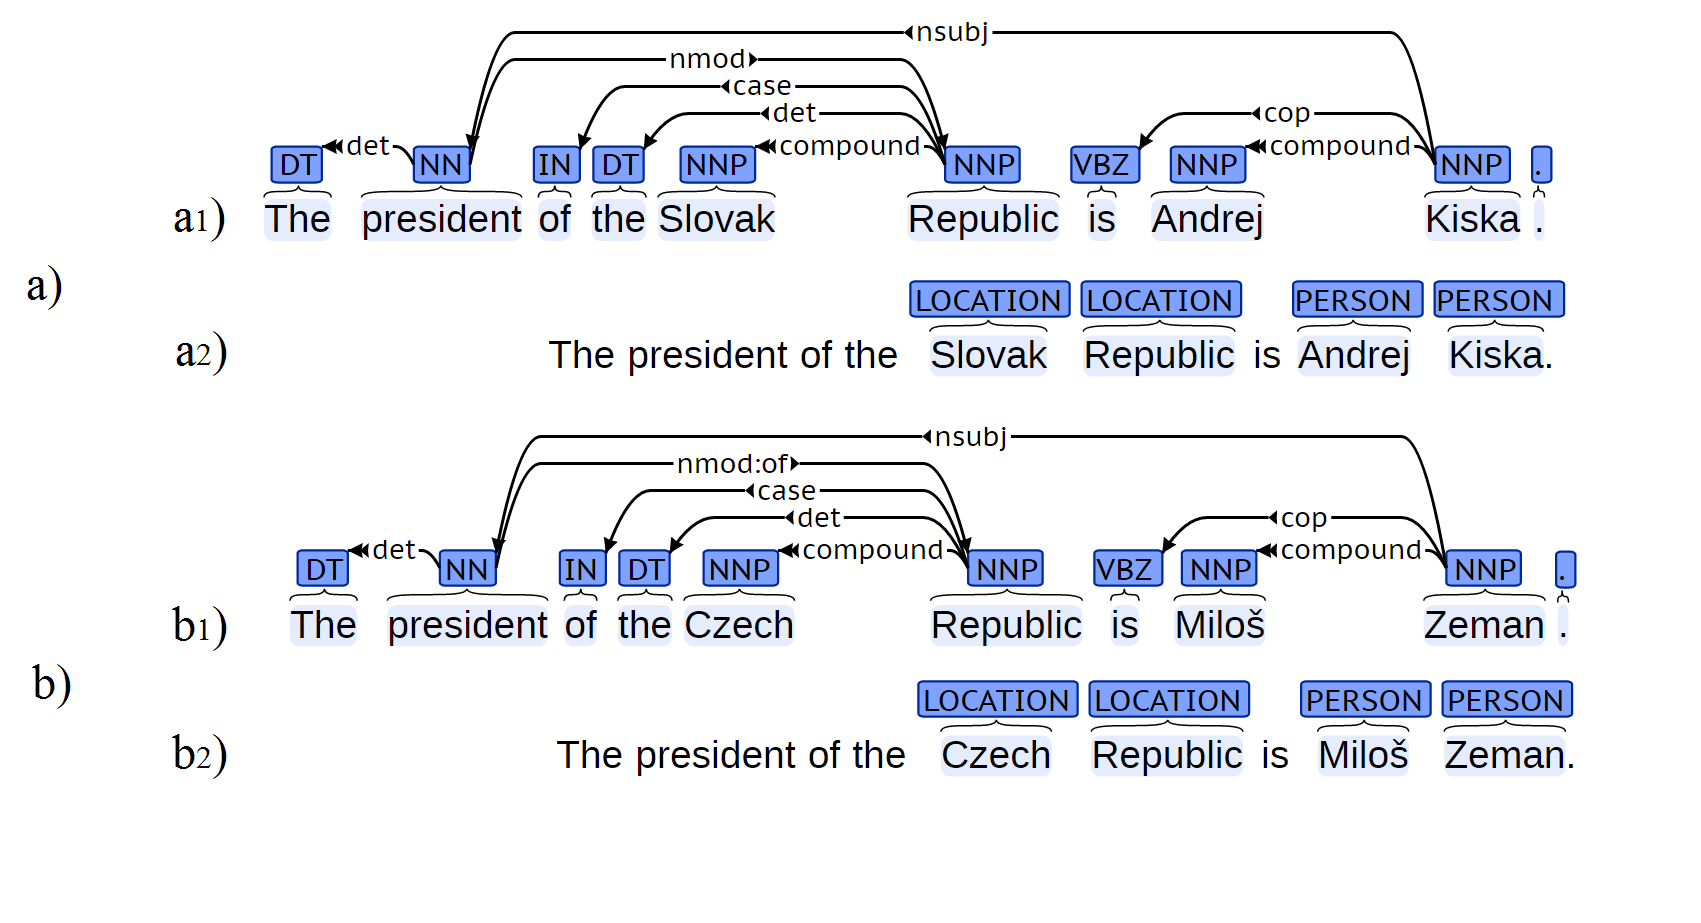
\includegraphics[scale=0.33]{calculate_sentences_match_example}\end{center}
	\caption[Príklad určenia zhody viet]{Príklad určenia zhody viet}\label{fig:calculate_match_sentences_example}
\end{figure}

Predpokladajme situáciu z obrázka~\fullref{fig:calculate_match_sentences_example}. V databáze máme uloženú spracovanú vetu \textit{a} aj s pravidlom pre túto vetu. Spracovávame vetu \textit{b}. Na časti \textit{a1} obrázka~\fullref{fig:calculate_match_sentences_example} sú znázornené závislostí a na časti \textit{a2} názvoslovné entity vety \textit{a}. Na časti \textit{b1} sú znázornené závislostí a na časti \textit{b2} názvoslovné entity vety \textit{b}. V tejto situácií potrebujeme vypočítať zhodu medzi vetami \textit{a} a \textit{b}. 

Pri štrukturálnej časti zhody sa prechádza cez všetky závislosti vety \textit{a}. Prvá závislosť je závislosť so vzťahom \textit{DET} a nadradeným tokenom s nadradenou značkou slovného druhu \textit{NN} a podradeným tokenom s nadradenou značkou slovného druhu \textit{DT}. V prom kroku sa pozrie, či veta \textit{b} obsahuje ľubovoľnú závislosť s podradeným tokenom s nadradenou značkou slovného druhu \textit{DT}. V ďalšom kroku, sa zistí, či veta \textit{b} obsahuje ľubovoľnú závislosť s nadradeným tokenom s nadradenou značkou sloveného druhu \textit{NN}. Môže to byť aj iná závislosť, ako tá z prvého kroku. Pokračuje sa zistením úplnej zhody závislosti. Určí sa , či veta \textit{b} obsahuje ľubovoľnú závislosť s podradeným tokenom s nadradenou značkou slovného druhu práve \textit{DT} a zároveň s nadradeným tokenom s nadradenou značkou slovného druhu \textit{NN}. Takto sa iteruje cez všetky závislosti vety \textit{a}. Na záver sa určí zhoda počtu závislostí s rovnakou štruktúrou. Napríklad veta \textit{a} obsahuje práve dve závislosti, ktoré majú na podradenom tokene nadradenú značku slového druhu \textit{DT} a na nadradenom tokene nadradenú značku slovného druhu \textit{NN}. Zistí sa, či aj veta \textit{b} obsahuje práve dve takéto závislosti. \\

Následne sa určuje obsahová časť zhody. Prvá závislosť vo vete \textit{b} je so vzťahom \textit{det}, nadradeným tokenom so značkou slovného druhu \textit{NN} a indexom 1 a podradeným tokenom so značkou slovného druhu \textit{DT} a indexom 0. Token slova \textit{Slovak} má názvoslovnú entity typu \textit{LOCATION - lokácia}. Ak slovo nemá vyobrazený typ názvoslovnej entity, znamená to, že má názvoslovnú entity typu \textit{OTHER - ostatné}. V prvok kroku pri určovaní obsahovej časti zhody zisťujeme, či veta \textit{b} obsahuje závislosť so vzťahom \textit{det} a tokenmi so značkou slovného druhu \textit{NN} alebo \textit{DT} a indexmi rovnými 0 alebo 1. Toto je separátny výpočet značiek slovných druhov a indexov. V tomto isto kroku sa tiež pozrie, či veta \textit{b} obsahuje ľubovoľnú závislosť s podradeným tokenon s názvoslovnou entitou typu \textit{ostatné} (názvoslovná entita tokenu \textit{THE} vo vete \textit{a}) a ľubovoľnú závislosť s nadradeným tokenom s názvoslovnou entitou typu \textit{ostatné} (názvoslovná entita tokenu \textit{president} vo vete \textit{a}). V nasledujúcom kroku zisťujeme, či veta \textit{b} obsahuje závislosť so vzťahom \textit{det} a nadradeným alebo podradeným tokenom so značkou slovného druhu \textit{NN} a indexom 1 alebo značkou slovného druhu \textit{DT} a indexom 0. Toto je polovičná zhoda. V poslednom kroku hľadáme vo vete \textit{b} závislosť so vzťahom \textit{det} a nadradeným tokenom práve so značkou slovného druhu \textit{NN} a indexom 1 a zároveň podradeným tokenom práve so značkou slovného druhu \textit{DT} a indexom 0. Zároveň v tomto kroku sa zisťuje, či veta \textit{b} obsahuje závislosť s podradeným tokenom s názvoslovnou entitou typu \textit{ostatné} a zároveň s nadradeným tokenom s názvoslovnou entitou typy \textit{ostatné}. Iterácia pokračuje s nasledujúcou závislosťou, pokým sa nevyhodnotia všetky. \\

Pri určení hodnotovej časti zhody sa porovnajú texty \textit{,,The president of the Slovak Republic is Andrej Kiska.''} a \textit{,,The president of the Czech Republic is Miloš Zeman.''} a určí sa, či su zhodné. \\

Aplikovaním určenia zhody viet medzi vetami \textit{a} a \textit{b} zistíme, že veta \textit{b} má štrukturálnu časť zhody s vetou \textit{a} $100\%$. Tak isto má obsahovú časť zhody rovnú $100\%$. Hodnotová časť zhody je $0\%$.

%
% Nadradená značka slovného druhu
%
\ifthenelse {\boolean{bachelor}}
{
	%\subsection{Subsection}
	\paragraph{Nadradená značka slovného druhu}
}
{
	%\section{Subsection}
	\subsubsection{Nadradená značka slovného druhu}
}
\label{paragraph:superior_pos_tag}

Pod nadradenou značkou slovného druhu sa chápe značka slovného druhu zoskupujúca množinu značiek slovných druhov, do ktorej značka slovného druhu patrí. 

Napríklad značka slovného druhu VBD (Verb, past tense - sloveso v minulom čase) patrí medzi skupinu značiek slovných druhov slovies \textit{\{VB, VBD, VBG, VBN, VBP, VBZ\}}. Z toho vyplýva, že nadradená značka slovného druhu \textit{VBD} je VB (Verb - sloveso).

%
% Aplikovanie pravidla
%
\ifthenelse {\boolean{bachelor}}
{
	%\subsection{Subsection}
	\subsubsection{Aplikovanie pravidla}
}
{
	%\section{Subsection}
	\subsection{Aplikovanie pravidla}
}
\label{subsubsection:rule_application}

Procesom vyhľadania pravidla (viď.~\fullref{subsubsection:rule_lookup}) sme získali pravidlo na spracovanie vety. Aplikáciou pravidla na vetu vytvoríme poznámku.

Proces aplikovania pravidla na vetu s cieľom vytvorenia poznámky má viacero krokov. Pre všetky závislosti zo \textit{zoznamu dát štruktúry} pravidla, príslušná závislosť je vyhľadaná v spracovávanej vete. Pri vyhľadávaní príslušnej závislosti sa závislosti neporovnávajú, okrem iného, na základe značiek slovných druhov svojich tokenov, ale podľa nadradených značiek slovných druhov (viď.~\nameref{paragraph:superior_pos_tag} na strane~\pageref{paragraph:superior_pos_tag}) svojich tokenov. Tento spôsob vyhľadávania nám umožňuje aplikovať jedno pravidlo na viacero viet, ako už bolo spomenuté v časti~\fullref{subsection:use_of_dependencies_in_notes_creation}. Avšak, môže to spôsobiť vyhľadanie viac ako jednej príslušnej závislosti. Preto musí byť vypočítaná zhoda závislostí (viď.~\nameref{paragraph:dependency_match} na strane \pageref{paragraph:dependency_match}). Po vypočítaní zhody závislostí a získaní závislosti s najväčšou zhodou, slovo korešpondujúce s tokenom, ktorý sa má z danej závislosti vybrať, sa pridá do poznámky na pozíciu pozície závislosti. Po spracovaní všetkých závislostí, posledné minoritné úpravy sú vykonané nad poznámkou, ako rozdelenie na viacero viet, ak tak určovalo pravidlo, kapitalizácia prvých písmen viet poznámky a iné. Pseudokód aplikovania pravidla na vetu s cieľom vytvoriť poznámku je zobrazený na algoritme~\ref{alg:applying_rule} Aplikovanie pravidla.

\begin{algorithm}
	\floatname{algorithm}{Algoritmus}
	\caption[Aplikovanie pravidla]{Aplikovanie pravidla}\label{alg:applying_rule}
	\begin{algorithmic}[1]
		\Procedure{AplikujPravidlo}{$veta, pravidlo$}
		\State $poznámka \gets \text{vytvor prázdnu poznámku}$
		\ForAll {$závislostí\text{ } v\text{ } pravidle$}
		\State $závislosť \gets \text{nájdiZávislosť(} veta \text{, } závislosť\text{ } pravidla \text{)}$
		\If {$závislosť \text{ existuje}$}
		\State $\text{pridaj } závislosť \text{ do } poznámky$
%		\If {$\text{isNominalSubject(relation(}dependency \text{))}$}
%		\State $\text{add(} note \text{, getGovernor(} dependency \text{))}$
		\EndIf
%		\EndIf
		\EndFor
		
		\State $\text{rozdeľ } poznámku \text{ na vety podľa } pravidla$	
		
		\Return $poznámka$
		\EndProcedure
	\end{algorithmic}
\end{algorithm}

Pre vetu \textit{,,The president of the Slovak republic is Andrej Kiska.''} nám nástroj Stanford CoreNLP poskytne závislostí vyobrazené na obrázku~\fullref{fig:example_sentence_andrej_kiska}. Ak na túto vetu aplikujeme pravidlo so štruktúrou v tvare zobrazenej na obrázku~\fullref{fig:apply_rule_example_rule}, výsledná poznámka bude \textit{,,President is Kiska.''}. 

Aplikovanie pravidla prebieha nasledovným spôsobom. Prechádzajú sa všetky závislosti v štruktúre pravidla. Prvá závislosť v štruktúre pravidla je závislosť so vzťahom \textit{nsubj} na pozícií jedna a podradeným korešpondujúcim tokenom. Má podradený token so značkou slovného druhu \textit{NN}, typom názvoslovnej entity \textit{OTHER - ostatné}, lemou \textit{President} a indexom dva. Nadradený token má značku slovného druhu \textit{NNP}, názvoslovnú entitu \textit{PERSON - osoba}, lemu \textit{Kiska} a index deväť. Takáto závislosť sa vyhľadá v štruktúre vety medzi závislosťami na obrázku~\fullref{fig:example_sentence_andrej_kiska}. Závislosti sa vyhľadávajú podľa zhody všetkých informácií o ich tokenoch a vzťahu medzi nimi. Ak pre danú závislosť vyhovuje viacero závislostí, pomocou výpočtu zhody závislostí vyberieme tú s najväčšou zhodou. V tomto prípade vidíme, že vyhovujúca závislosť je len jedna a to prvá závislosť \textit{nsubj} medzi slovom na druhej pozícií \textit{president} a posledným slovom, na deviatej pozícií \textit{Kiska}. Z tejto závislosti sa zoberie podradený token, keďže tak určuje pravidlo v stĺpci \textit{typ tokenu}. Slovo \textit{president} sa pridá do poznámky na pozíciu jedna. Rovnakým spôsobom sa prechádzajú a spracujú všetky závislosti v štruktúre pravidla a podľa nich sa extrahuje slovo z vety a pridá do poznámky.

\begin{figure}[H]
	\begin{center}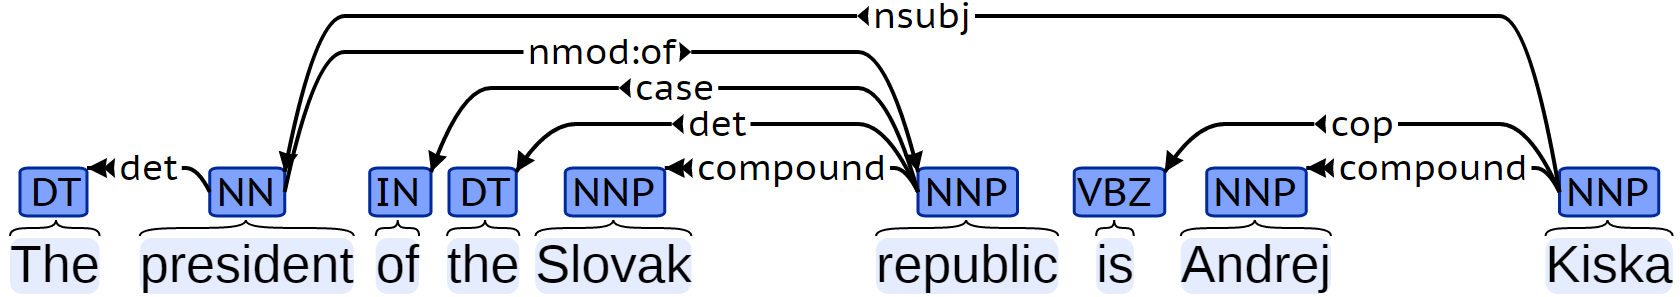
\includegraphics[scale=0.31]{example_sentence_andrej_kiska}\end{center}
	\caption[Závislostí jednoduchej vety]{Závislostí jednoduchej vety}\label{fig:example_sentence_andrej_kiska}
\end{figure}

\begin{figure}[H]
	\begin{center}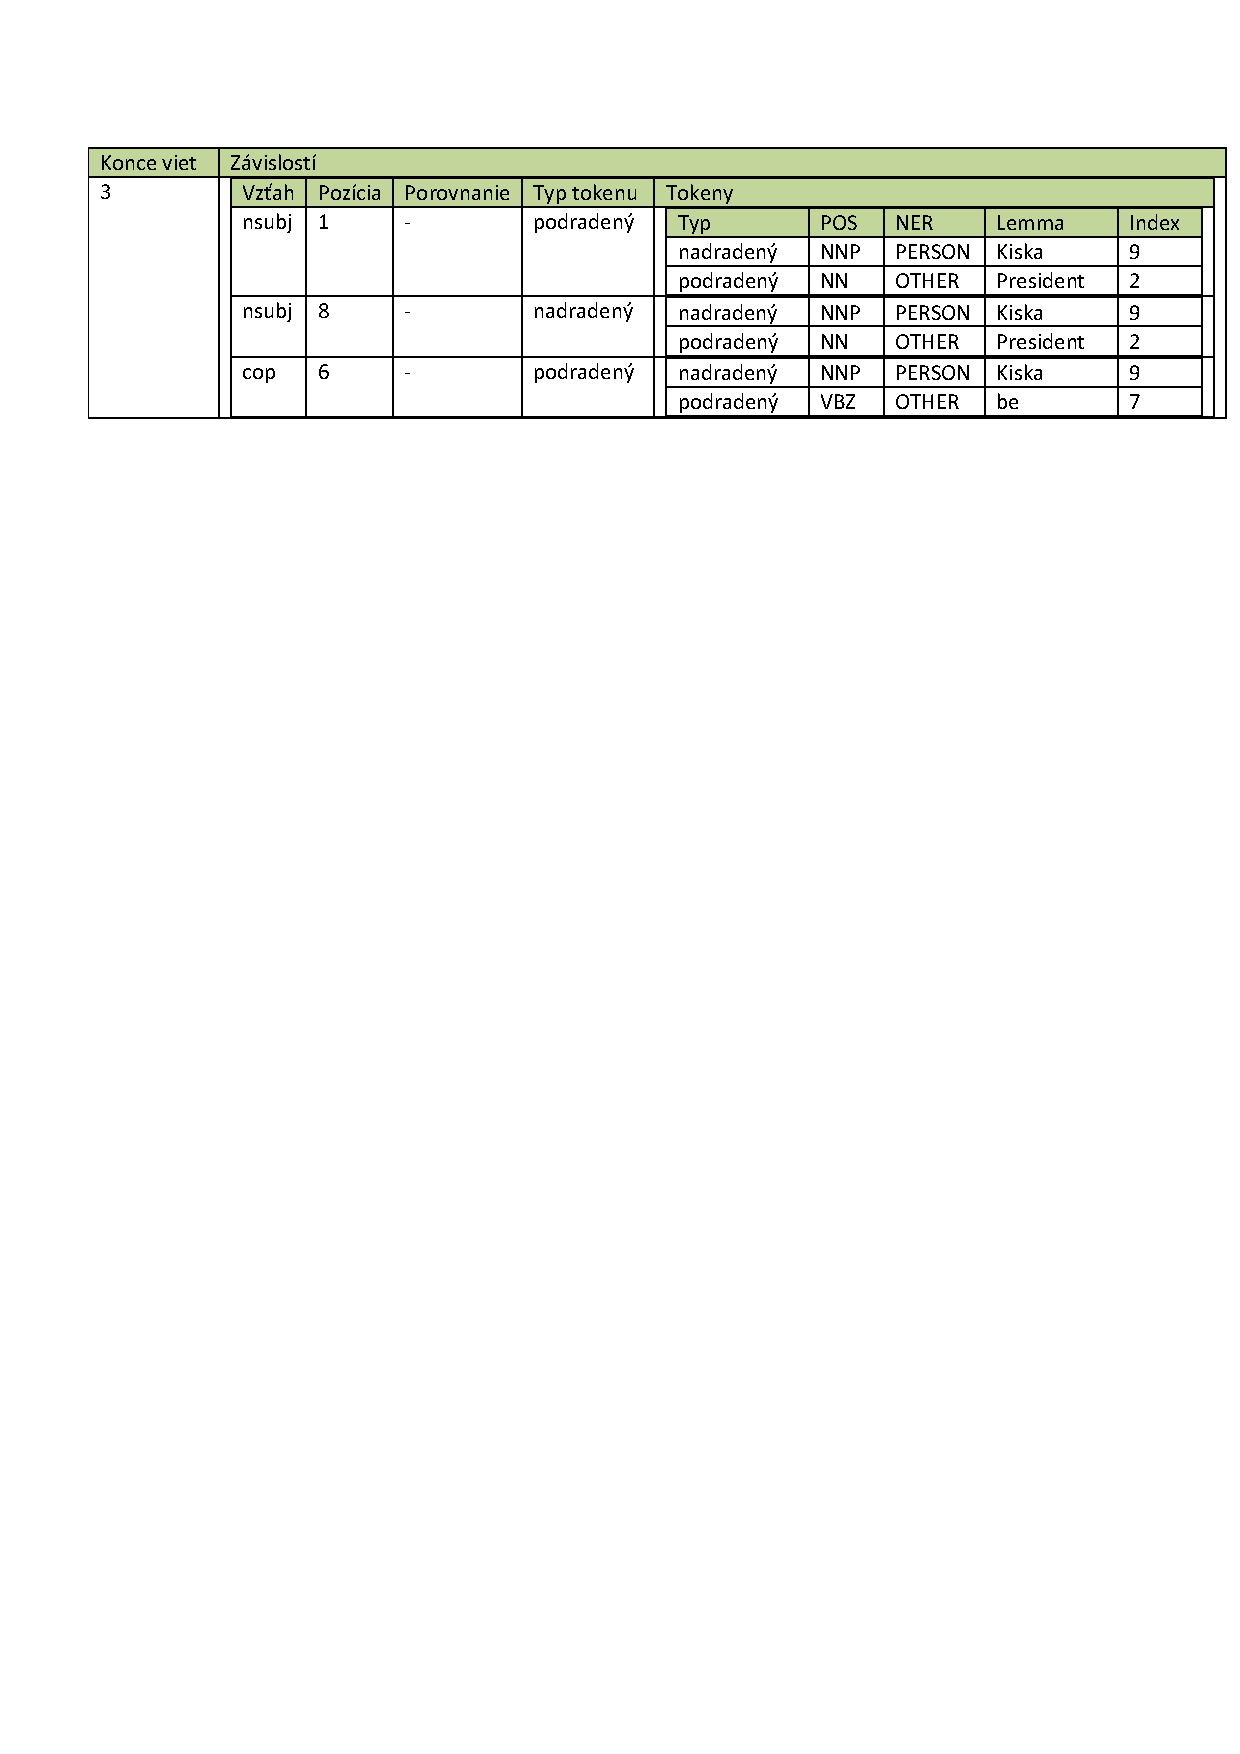
\includegraphics[scale=0.32]{apply_rule_example_rule}\end{center}
	\caption[Príklad štruktúry pravidla]{Príklad štruktúry pravidla}\label{fig:apply_rule_example_rule}
\end{figure}

%
% Výpočet zhody závislostí
%
\ifthenelse {\boolean{bachelor}}
{
	%\subsection{Subsection}
	\paragraph{Výpočet zhody závislostí}
}
{
	%\section{Subsection}
	\subsubsection{Výpočet zhody závislostí}
}
\label{paragraph:dependency_match}

Princíp výpočtu zhody závislostí je veľmi podobný s výpočtom zhody viet zo sekcie~\fullref{subsubsection:rule_lookup}. Porovnávajú sa vždy nadradené aj podradené tokeny. Porovnanie má niekoľko krokov. Začína sa s porovnaním značiek slovných druhov. Pokračuje sa názvoslovnou entitou, indexom, lemou a nakoniec sa porovnáva vzdialenosť pozícií tokenov vo vetách. Každý krok je príslušne ohodnotený a ak porovnanie bolo úspešné, ohodnotenie sa pripočíta k finálnej hodnote reprezentujúcej percentuálnej zhody závislostí.

%
% Vytváranie pravidla
%
\ifthenelse {\boolean{bachelor}}
{
	%\subsection{Subsection}
	\subsubsection{Vytvorenie pravidla}
}
{
	%\section{Subsection}
	\subsection{Vytvorenie pravidla}
}
\label{subsubsection:rule_creation}
Ak nám proces vyhľadania pravidla nevyhľadal žiadne pravidlo, znamená to, že sme doposiaľ nespracovávali takú istú alebo podobnú vetu. V tomto prípade sú použité statické pravidlá na spracovanie vety. Výstupom bude poznámka.

Zo závislostí pôvodnej vety a informácií o ich tokenoch sa vytvorí nový záznam o štruktúre pôvodnej vety. Tak isto sa vytvorí aj nový záznam o štruktúre poznámky. Z poznámky sa vytvorí záznam o novej poznámke a následne sa z nej vytvorí zoznam koncov viet. Tento zoznam spolu so štruktúrou poznámky vytvorí záznam nového pravidla. Z pôvodnej vety sa vytvorí záznam o vete a prepojí sa so štruktúrou pôvodnej vety, článkom, ktorý obsahoval danú vetu a pravidlom, ktoré bolo vytvorené a použité a s poznámkou, ktorá vznikla z vety. Týmto vznikne nové pravidlo na spracovanie takej istej alebo podobnej vety ako sme práve spracovali.

%Na obrázku~\fullref{fig:rule_creation} je znázornený proces nevyhľadania pravidla, použitia parsera s následným uložením nového pravidla.

%\begin{figure}[H]
%	\begin{center}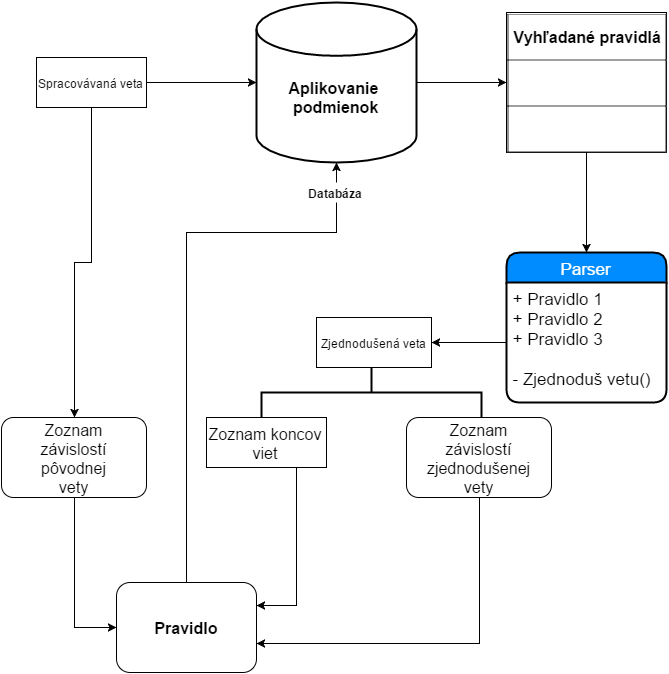
\includegraphics[scale=0.5]{rule_creation}\end{center}
%	\caption[Vytvorenie pravidla]{Vytvorenie pravidla}\label{fig:rule_creation}
%\end{figure}

%
% Úprava pravidla
%
\ifthenelse {\boolean{bachelor}}
{
	%\subsection{Subsection}
	\subsubsection{Úprava pravidla}
}
{
	%\section{Subsection}
	\subsection{Update rule}
}
\label{subsubsection:rule_update}
Systém umožňuje používateľovi upraviť vytvorenú poznámku. Tá sa da upraviť z množiny slov pôvodnej vety, pričom sa dajú ľubovoľne usporiadať a definovať ľubovoľný počet viet, na ktoré poznámku rozdeliť. Úpravou poznámky sa systém ,,naučí'' nové pravidlo alebo upraví existujúce pravidlo. Ktorá z týchto dvoch akcií sa vykoná sa rozhoduje podľa zhody, ktorá bola určená pri spracovávaní pôvodnej vety poznámky. 

Ak je štrukturálna časť zhody  menšia ako $100\%$, tým pádom aj obsahová a hodnotová zhoda je pod $100\%$, tak sa systém naučí nové pravidlo. Znamená to, že systém doposiaľ nespracovával vetu s rovnakou štruktúrou, a tak použil pravidlo podľa vety s najpodobnejšou štruktúrou a po úprave poznámky sa naučí, ako spracovať vetu s danou štruktúrou.

V prípade, že štrukturálna čast zhody je $100\%$, ale obsahová nie je úplná a tým pádom ani hodnotová, znamená to, že systém spracoval vetu s rovnakou štruktúrou, ale iným obsahom. V tomto prípade systém pozná ako spracovať vetu s danou štruktúrou, takže sa štruktúra pravidla upraví podľa vykonaných zmien. Vytvorí sa nový záznam o poznámke a aj o pôvodnej vete a prepoja sa na upravené pravidlo, pomocou ktorého bude systém vedieť spracovať viacero viet.

Pri $100\%$ štrukturálnej, obsahovej aj hodnotovej časti zhody, systém spracoval identickú vetu, akú už v minulosti spracoval. Preto sa zmeny na vytvorenej poznámke prejavia pri upravení pravidla. Tak isto sa upraví aj vytvorená poznámka, aby reflektovala vykonané zmeny.

%
% Priestor na rozvoj
%
\ifthenelse {\boolean{bachelor}}
{
	%\subsection{Subsection}
	\subsection{Priestor na rozvoj}
}
{
	%\section{Subsection}
	\section{Priestor na rozvoj}
}
\label{subsection:system_continue}
Systém ponúka priestor na jeho ďalší vývoj. Dostupných je niekoľko oblastí, v ktorých by sa dal ďalej rozvíjať.

Aby bolo vytváranie poznámok čo najefektívnejšie, je potrebné vstupný text predspracovať. Elimináciou nepodstatných častí textu, konkrétne viet, by sa výrazne zredukoval počet viet, ktoré musí systém alebo používateľ spracovať. Eliminácia nepodstatných viet by nemusela vykonávať známymi algoritmami, ale mohla by sa vykonávať napríklad na základe kľúčových slov v poznámkach. Podľa toho ako by si používateľ upravoval poznámky a tým definoval pravidla, by sa systém vedel naučiť podľa výskytu kľúčových slov v poznámkach, ktoré informácie sú pre používateľa dôležité. Na základe toho by vedel určiť dôležitosť vety pre používateľa a eliminovať ju ak by nevyhovovala rozmedziu, ktoré by stanovovalo, ktoré vety eliminovať, a ktoré nie.

Ďalšou oblasťou rozvoja by mohlo byť definovanie si vlastných závislostí. Vďaka vlastným závislostiam by nebol systém odkázaný na závislostí slov vo vete a hľadaní vzoru vo vetách na vytvorenie poznámky. Mohol by byť modifikovaný na hľadanie iných vzorov, napríklad vo vetách.

%
% Zhrnutie
%
\ifthenelse {\boolean{bachelor}}
{
	%\subsection{Subsection}
	\subsection{Zhrnutie}
}
{
	%\section{Subsection}
	\section{Summary}
}
\label{subsection:system_summary}
Dummy text..